\documentclass[conference]{IEEEtran}
\usepackage{cite}
\usepackage{amsmath,amssymb}
\usepackage{graphicx}
\usepackage{booktabs}
\usepackage{multirow}
\usepackage{xcolor}
\usepackage{url}
\graphicspath{{figs/}}

% ---------------------------------------------------------------- macros (edit numbers here)
\newcommand{\Ctot}{20~Mbps}
\newcommand{\Nunits}{100}

\begin{document}

\title{Adaptive 5G Resource Allocation and QoS Optimization:\\
Learning-Driven Adaptive Network Slicing for eMBB, URLLC and mMTC Traffic}

\author{\IEEEauthorblockN{Sai Govardhan Rao Medikurthi}
\IEEEauthorblockA{IT365 Advanced Computer Networks\\
National Institute of Technology Karnataka, Surathkal}
\and
\IEEEauthorblockN{Avulakonda Siva Sai}
\IEEEauthorblockA{IT365 Advanced Computer Networks\\
National Institute of Technology Karnataka, Surathkal}}

\maketitle

% =====================================================================
\begin{abstract}
5G networks multiplex enhanced Mobile Broadband (eMBB), Ultra-Reliable Low-Latency Communication (URLLC) and massive Machine-Type Communication (mMTC) traffic over shared resources by partitioning them into network slices. A fixed partition is simple but cannot follow traffic that changes over time. This paper presents the first half of a project that investigates learning-based adaptive slicing. We build an ns-3 simulation in which three slices share a pool of \Nunits{} resource units (\Ctot{}), each slice receiving a dedicated, run-time reconfigurable rate pipe with an explicit FIFO queue. Three UEs generate constant-bit-rate eMBB traffic, three UEs generate Poisson URLLC traffic, and up to 60 mMTC devices generate Poisson sensor traffic across a five-phase, 50~s scenario. Under a static 50/30/20 allocation, averaged over five seeds, the network leaves on average 27.8\% of the capacity unused while other slices drop traffic: eMBB loses 29.6\% of its packets during its burst while 5.4~Mbps sits idle in other slices; during a URLLC surge 99.9\% of URLLC packets exceed the 10~ms delay budget and 41.8\% are lost while 6.6~Mbps is idle; and only 32.5 of 60 mMTC devices are served during a device surge. Measured delays agree with M/D/1 and full-buffer queueing estimates, which validates the model. We then specify the complete post-midsem design: a Deep Q-Network (DQN) controller connected to ns-3 through shared memory, its state, action set, multi-objective reward, training protocol and evaluation plan. Only static-baseline results are reported here; no learning results are claimed.
\end{abstract}

\begin{IEEEkeywords}
5G, network slicing, eMBB, URLLC, mMTC, ns-3, QoS, resource allocation, deep reinforcement learning, DQN
\end{IEEEkeywords}

% =====================================================================
\section{Introduction}
IMT-2020 defines three usage scenarios with very different requirements \cite{itu2083}: eMBB needs high throughput, URLLC needs low latency with high reliability, and mMTC needs to support a very large number of low-rate devices. Network slicing lets an operator run logically isolated networks for these services on shared infrastructure \cite{ts23501,foukas2017}. The question this project addresses is \emph{how much of the shared resource each slice should receive at each moment}.

A static partition is the simplest answer, and it works while traffic stays close to the design point. Real traffic is bursty. When one slice bursts above its share, its packets queue and are dropped, even if another slice is lightly loaded at the same time. The result is the combination this paper measures: QoS violations in one slice and unused capacity in another.

The project is split into two phases. \textbf{Phase~1 (this midsem report)} builds a working ns-3 slicing simulation with a real, enforced resource partition, a dynamic traffic scenario, per-interval QoS measurement and a static baseline. \textbf{Phase~2} adds a DQN controller that changes the partition during the simulation. The contributions of this report are:
\begin{itemize}
\item An ns-3 model of rate-based slicing in which each slice's share is enforced by a dedicated pipe whose rate can be changed at run time through a single function, \texttt{ApplyAllocation()}, which later becomes the RL action.
\item A five-phase traffic scenario and a measurement layer that records throughput, mean and 95th-percentile delay, packet loss, URLLC violations, served mMTC devices and utilisation every 100~ms.
\item A quantified static baseline over five seeds, validated against queueing theory, showing simultaneous under-utilisation and QoS violation.
\item A complete design for the adaptive controller (state, actions, reward, DQN training, ns-3 to Python interface, comparison protocol and dashboard).
\end{itemize}

% =====================================================================
\section{Background and Related Work}
\subsection{Slices and their requirements}
3GPP specifies slice/service types for eMBB, URLLC and MIoT (massive IoT) \cite{ts23501}, and service-level targets in \cite{ts22261}. The 1~ms URLLC latency figure in the literature refers to the radio user plane \cite{itu2083}. Popovski \emph{et al.} \cite{popovski2018} analyse the three services from a communication-theoretic view and show that their resource needs are fundamentally different, which motivates per-slice isolation.

\subsection{Learning-based slicing}
Deep reinforcement learning (DRL) has been applied to slice resource management, where an agent observes demand and QoS and chooses a resource split \cite{li2018}. The DQN algorithm \cite{mnih2015} is a common starting point because the action set can be kept small and discrete.

\subsection{Simulation tools}
ns-3 \cite{ns3} is a discrete-event packet-level simulator widely used in networking research. 5G-LENA \cite{lena2019} adds a full 5G NR stack. ns3-gym \cite{ns3gym} and ns3-ai \cite{ns3ai} connect ns-3 to Python ML frameworks; ns3-ai uses shared memory and is faster for per-step interaction.

% =====================================================================
\section{System Model and Methodology}

\subsection{Design choice: abstraction instead of a full NR stack}
A full 5G-LENA model would add PHY/MAC detail (numerology, HARQ, channel models, schedulers) that is not needed to study the allocation question, and would make every simulation step much slower, which matters when the RL agent needs thousands of steps. We therefore model each slice's share of the radio resource as a \emph{rate pipe} (Section~\ref{sec:res}). This is a documented abstraction: a resource unit in this paper is \textbf{not} a physical resource block (PRB). The abstraction keeps the networking behaviour that matters here (capacity sharing, queueing, delay, loss) and can later be replaced by 5G-LENA without changing the controller.

\subsection{Topology}
Fig.~\ref{fig:topo} shows the topology, built with the ns-3 \texttt{point-to-point}, \texttt{internet}, \texttt{traffic-control} and \texttt{applications} modules. Traffic is uplink. Each user equipment (UE) connects to its slice gateway over a 100~Mbps, 0.1~ms access link, which is never the bottleneck. Each gateway connects to the base station (BS) over a \emph{slice pipe} with 1~ms propagation delay. The BS hosts one UDP sink per slice and timestamps every packet.

\begin{figure}[t]
\centering
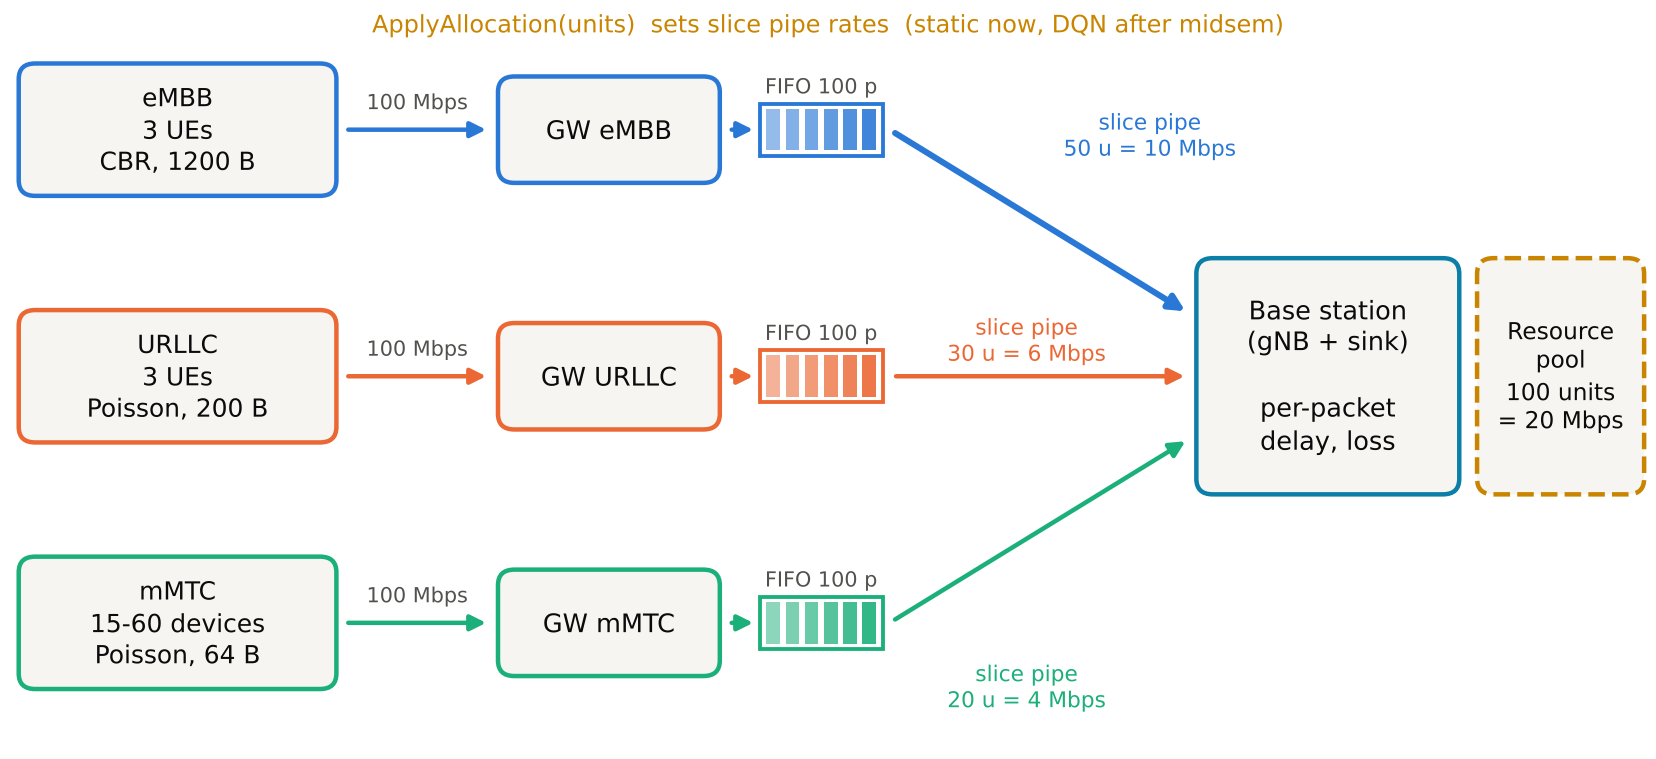
\includegraphics[width=\columnwidth]{arch_topology.png}
\caption{Simulated topology. Each slice owns a pipe whose rate equals its allocated share of the 100-unit (\Ctot{}) pool; each pipe has an explicit 100-packet FIFO.}
\label{fig:topo}
\end{figure}

\subsection{Resource model}\label{sec:res}
The shared capacity $C=\Ctot$ is divided into $N=\Nunits$ units, so one unit is $C/N=0.2$~Mbps. An allocation is a vector $\mathbf{a}=(a_e,a_u,a_m)$ with
\begin{equation}
a_e+a_u+a_m=N,\qquad C_k=a_k\,\frac{C}{N},\quad k\in\{e,u,m\},
\end{equation}
where $C_k$ is the rate of slice $k$'s pipe. \texttt{ApplyAllocation}$(\mathbf{a})$ sets the data rate of both ends of each pipe during the simulation. Slices are strictly isolated: unused capacity in one pipe cannot be borrowed by another. This is the defining property of a static hard partition, and it is what an adaptive controller can improve on.

\subsection{Queueing}
Each pipe has an explicitly installed \texttt{FifoQueueDisc} with a 100-packet limit and a 1-packet device queue. The queue disc is installed before IP address assignment, so ns-3's default \texttt{FqCoDel} queue disc is not used on the pipes. Without this step the default fair queue would silently redistribute capacity and mask the allocation being studied.

\subsection{Traffic model}
\begin{itemize}
\item \textbf{eMBB:} 3 UEs, constant bit rate, 1200-byte UDP payloads (video-like).
\item \textbf{URLLC:} 3 UEs, Poisson arrivals, 200-byte payloads (control messages).
\item \textbf{mMTC:} up to 60 devices, each Poisson at 100 packets/s with 64-byte payloads (sensor reports); a phase activates a subset of devices.
\end{itemize}
Every payload carries a 12-byte sequence/timestamp header. IPv4, UDP and PPP add 30~bytes, so the load on the wire is higher than the payload rate (by 15\% for URLLC and 47\% for mMTC); all capacity comparisons below use wire rates. Table~\ref{tab:phases} lists the five phases.

\begin{table}[t]
\centering
\caption{Traffic scenario (payload load; wire load in brackets)}
\label{tab:phases}
\footnotesize
\setlength{\tabcolsep}{2.5pt}
\begin{tabular}{@{}llccc@{}}
\toprule
Phase & Time & eMBB Mbps & URLLC Mbps & mMTC devs \\
\midrule
P1 Normal & 0 to 10 s & 6 [6.15] & 2 [2.30] & 30 [2.26] \\
P2 eMBB burst & 10 to 20 s & 14 [14.35] & 2 [2.30] & 30 [2.26] \\
P3 eMBB+URLLC & 20 to 30 s & 14 [14.35] & 5 [5.75] & 30 [2.26] \\
P4 URLLC v.\ high & 30 to 40 s & 6 [6.15] & 9 [10.35] & 15 [1.13] \\
P5 mMTC surge & 40 to 50 s & 9 [9.22] & 2 [2.30] & 60 [4.51] \\
\bottomrule
\end{tabular}
\end{table}

\subsection{Static baseline}
The baseline allocation is $\mathbf{a}=(50,30,20)$ units, i.e.\ 10, 6 and 4~Mbps for eMBB, URLLC and mMTC, held constant for the whole run.

\subsection{Metrics}\label{sec:metrics}
Statistics are collected in bins of $\Delta=100$~ms. For slice $k$ in bin $t$: throughput $T_k(t)$ is received payload bits divided by $\Delta$; delay is the one-way delay from the packet timestamp, reported as mean and 95th percentile; loss is computed by \emph{transmit} bin,
\begin{equation}
L_k(t)=1-\frac{\#\{\text{packets sent in }t\text{ and later delivered}\}}{\#\{\text{packets sent in }t\}},
\end{equation}
so packets still queued are not miscounted as lost. The URLLC violation ratio $V(t)$ is the fraction of URLLC packets received in bin $t$ with delay above a budget $D_{\max}=10$~ms. With 1.1~ms of fixed propagation delay in the model, the 3GPP 1~ms radio target cannot apply end to end, so $D_{\max}$ is a simulation budget, not a standard value. An mMTC device is \emph{served} in a bin if at least 90\% of the packets it sent in that bin are delivered. Slice utilisation is wire throughput over $C_k$. Finally, per phase we report the capacity left unused in under-loaded slices and the demand dropped in over-loaded slices:
\begin{align}
U_{\text{idle}}&=\textstyle\sum_k \max(C_k-\text{carried}_k,0),\\
U_{\text{unmet}}&=\textstyle\sum_k \max(\text{offered}_k-\text{carried}_k,0).
\end{align}
When $U_{\text{unmet}}\le U_{\text{idle}}$, a better allocation of the same total capacity could have carried all traffic.

Each configuration is run with five random seeds (ns-3 run numbers 1 to 5); we report means and 95\% confidence intervals.

\subsection{Adaptive controller design (Phase~2)}
This subsection specifies the controller that will be implemented after midsem. Fig.~\ref{fig:sys} shows the full architecture; solid blocks exist now, dashed blocks are Phase~2.

\begin{figure*}[t]
\centering
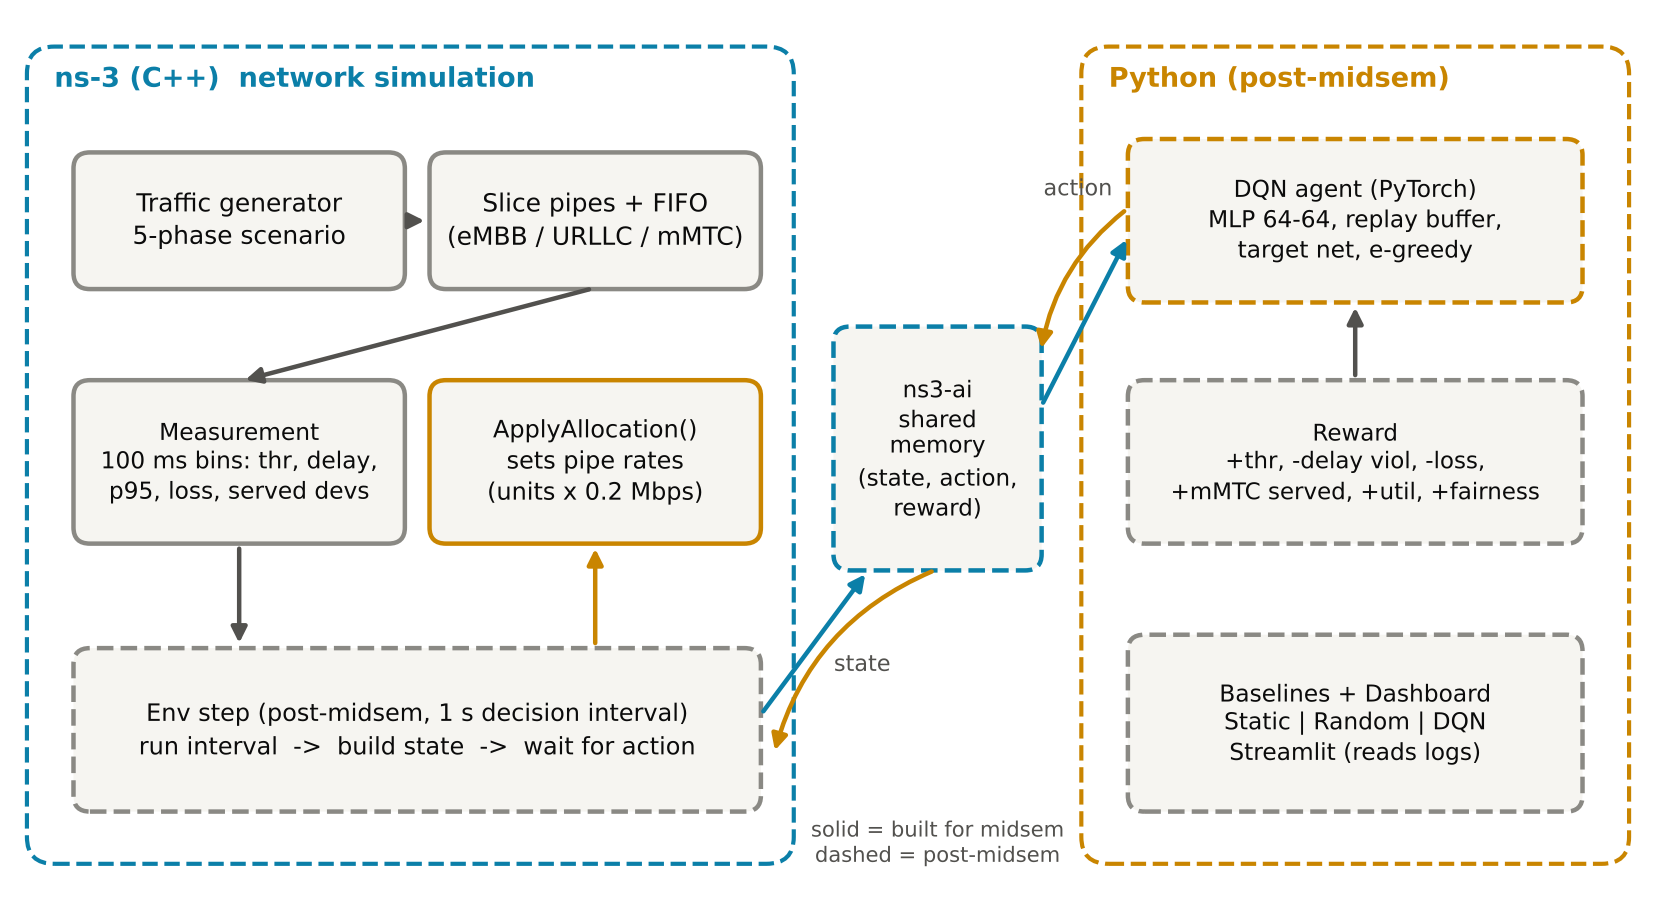
\includegraphics[width=0.82\textwidth]{arch_system.png}
\caption{End-to-end architecture. The ns-3 simulation (left) exposes state and accepts an allocation each decision interval through ns3-ai shared memory; the DQN agent, reward computation, baselines and dashboard run in Python (right).}
\label{fig:sys}
\end{figure*}

\subsubsection{Control loop and interface}
The decision interval is $\tau=1$~s (10 measurement bins). At each step ns-3 runs for $\tau$, aggregates the bins into a state vector, writes it to shared memory via ns3-ai \cite{ns3ai}, and blocks. The Python agent reads the state, computes the reward of the previous action, chooses a new allocation and writes it back; ns-3 calls \texttt{ApplyAllocation()} and continues. An episode is one 50~s scenario, i.e.\ 50 steps. ns3-gym \cite{ns3gym} is a drop-in alternative with a socket interface.

\subsubsection{State}
A 10-dimensional vector, each element scaled to roughly $[0,1]$: offered load of each slice divided by $C$ (3); current allocation $a_k/N$ (3); eMBB delivered/offered ratio; URLLC 95th-percentile delay divided by $D_{\max}$; URLLC loss ratio; and the fraction of active mMTC devices served. Offered load is measured at the gateways; in a real RAN the equivalent signal is the buffer status reported by UEs.

\subsubsection{Action space}
The action is a full allocation. The proposal's five actions cap URLLC at 50 units (10~Mbps), but the baseline results show that phase P4 needs 10.35~Mbps of wire capacity, i.e.\ at least 52 units. The action set is therefore all allocations in steps of 10 units with every slice receiving at least 10 units, which gives 36 actions including URLLC shares of up to 80 units. The step size can be refined if the experiments require it.

\subsubsection{Reward}
\begin{equation}
\begin{split}
r_t ={}& w_1\,\bar T_e(t) - w_2\,V(t) - w_3\,\textstyle\sum_k \lambda_k L_k(t)\\
&+ w_4\,S_m(t) + w_5\,\eta(t) + w_6\,J(t) - w_7\,\mathbb{1}[\mathbf{a}_t\neq\mathbf{a}_{t-1}],
\end{split}
\end{equation}
where $\bar T_e$ is eMBB throughput normalised by its offered load, $V$ the URLLC violation ratio, $L_k$ the per-slice loss with priority weights $\lambda_u>\lambda_e>\lambda_m$, $S_m$ the served mMTC fraction, $\eta$ the total utilisation, and $J$ Jain's fairness index \cite{jain1984} over the per-slice satisfaction ratios (carried/offered). The last term discourages needless switching. The starting weights are $(w_1,\dots,w_7)=(1,5,2,1,0.5,0.5,0.1)$, so that a URLLC violation costs the most. They will be tuned with a small sweep on training scenarios and reported with that sweep, so that the choice is justified experimentally rather than assumed.

\subsubsection{DQN}
The Q-network is a multilayer perceptron with input 10, two hidden layers of 64 ReLU units and 36 outputs, one Q-value per action. It is trained with the standard DQN loss \cite{mnih2015}
\begin{equation}
\mathcal{L}(\theta)=\mathbb{E}\Big[\big(r+\gamma\max_{a'}Q_{\theta^-}(s',a')-Q_\theta(s,a)\big)^2\Big],
\end{equation}
using an experience replay buffer of 20\,000 transitions, minibatches of 64, a target network $\theta^-$ copied every 200 steps, Adam with learning rate $10^{-3}$, discount $\gamma=0.9$, and $\varepsilon$-greedy exploration decayed from 1.0 to 0.05. Training uses 300 to 500 episodes. To prevent the agent from memorising one fixed trace, phase order, burst levels and burst start times are randomised in each training episode.

\subsubsection{Evaluation protocol}
Three controllers are run on identical held-out scenarios and seeds: Static (50/30/20), Random (uniform over the action set each step), and DQN. A demand-proportional heuristic is recommended as an additional reference, because a learned controller should also beat a simple rule. Five experiments are planned: normal traffic, eMBB burst, URLLC burst, mMTC device surge, and a highly dynamic mix. The metrics are those of Section~\ref{sec:metrics} plus Jain's fairness index, each with 95\% confidence intervals over seeds.

\subsubsection{Dashboard and extension}
A Streamlit dashboard reads the logged time series and shows current traffic, allocation, per-slice QoS, utilisation, fairness and violations, with Static and DQN side by side. As an optional extension, a moving-average or LSTM forecast of next-interval demand is appended to the state, and the reactive DQN is compared with the forecast-assisted DQN.

% =====================================================================
\section{Results: Static Baseline}
All results in this section come from the implemented ns-3 simulation (ns-3.44, five seeds, about 341\,000 packets per run). Fig.~\ref{fig:demand} to Fig.~\ref{fig:stranded} show seed-averaged time series smoothed over 0.5~s; Table~\ref{tab:summary} gives per-phase values.

\begin{figure}[t]
\centering
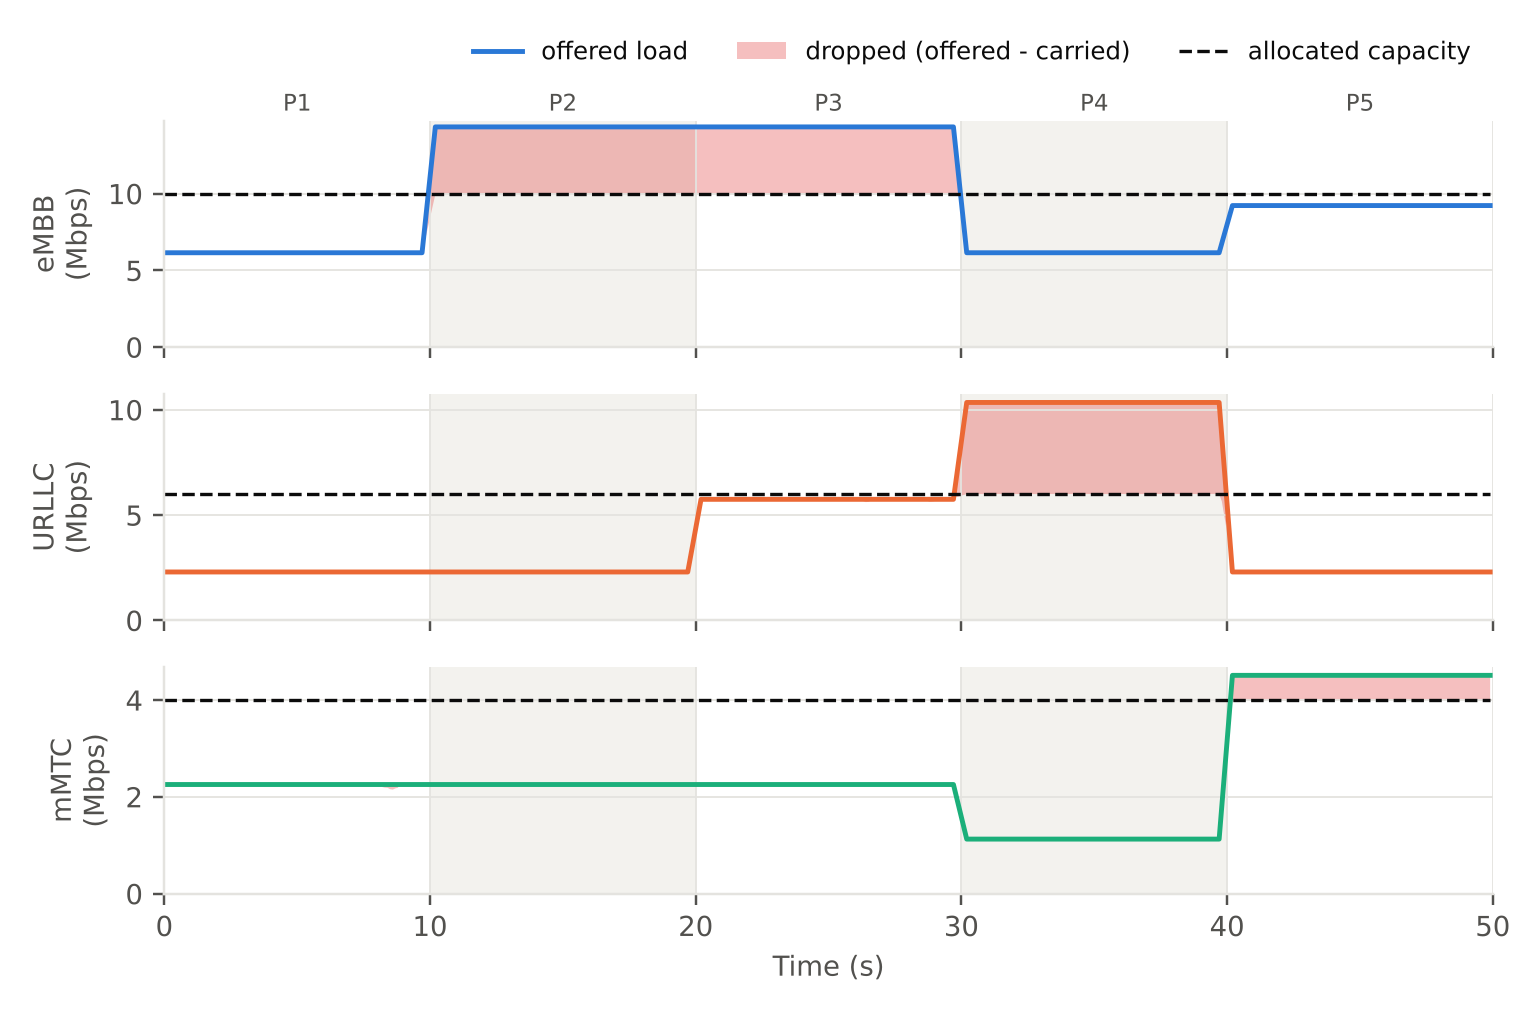
\includegraphics[width=\columnwidth]{fig1_demand_vs_capacity.png}
\caption{Offered wire load versus allocated capacity per slice. Shaded areas are traffic dropped because offered load exceeds the slice's fixed share.}
\label{fig:demand}
\end{figure}

\begin{figure}[t]
\centering
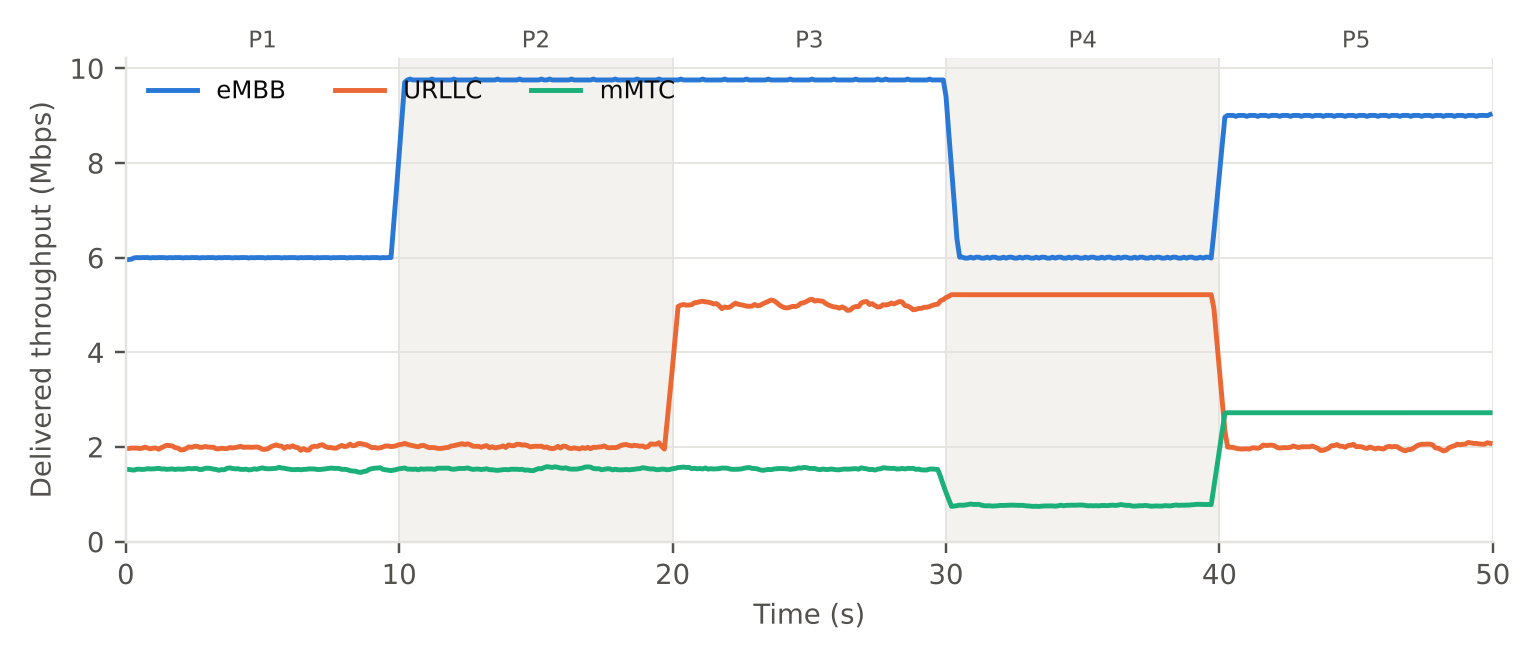
\includegraphics[width=\columnwidth]{fig2_throughput.png}
\caption{Delivered payload throughput per slice. eMBB is capped at its pipe rate in P2 and P3, and URLLC in P4.}
\label{fig:thr}
\end{figure}

\begin{figure}[t]
\centering
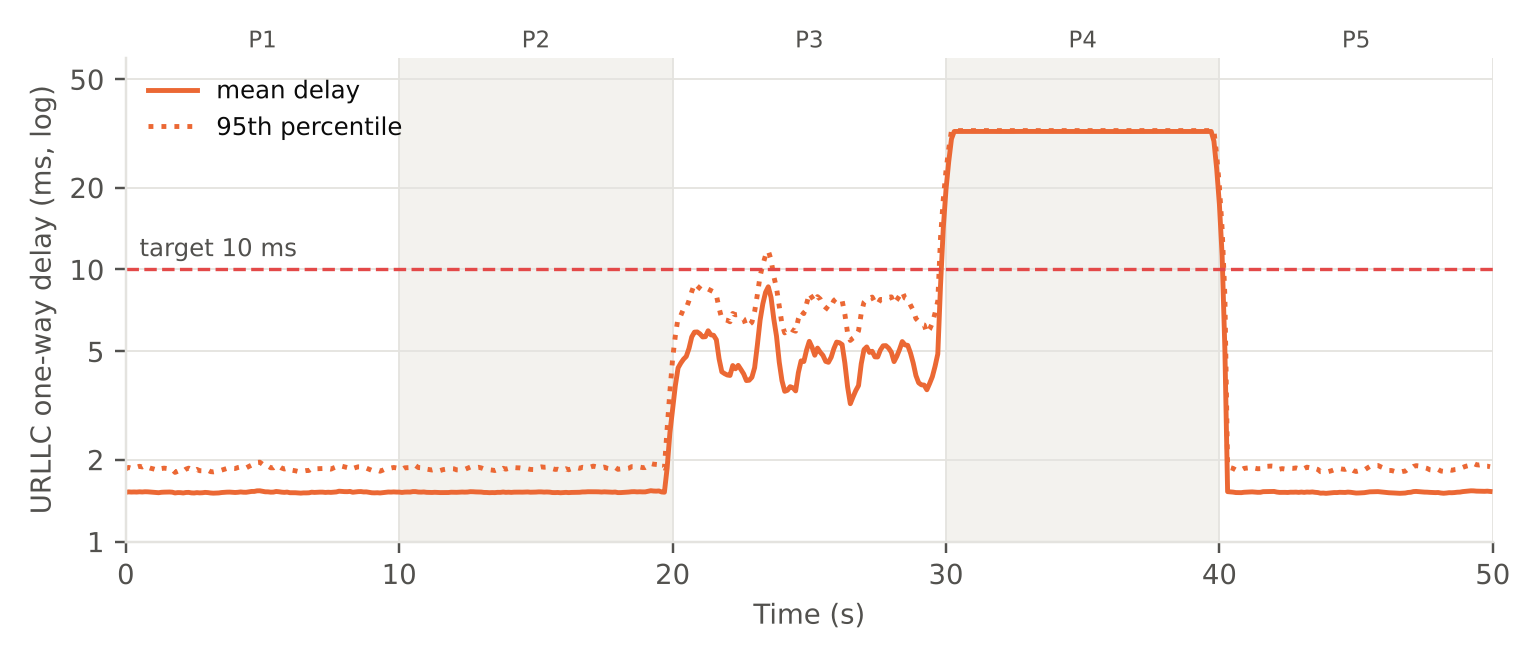
\includegraphics[width=\columnwidth]{fig3_urllc_latency.png}
\caption{URLLC one-way delay (log scale): mean and 95th percentile against the 10~ms budget.}
\label{fig:lat}
\end{figure}

\begin{figure}[t]
\centering
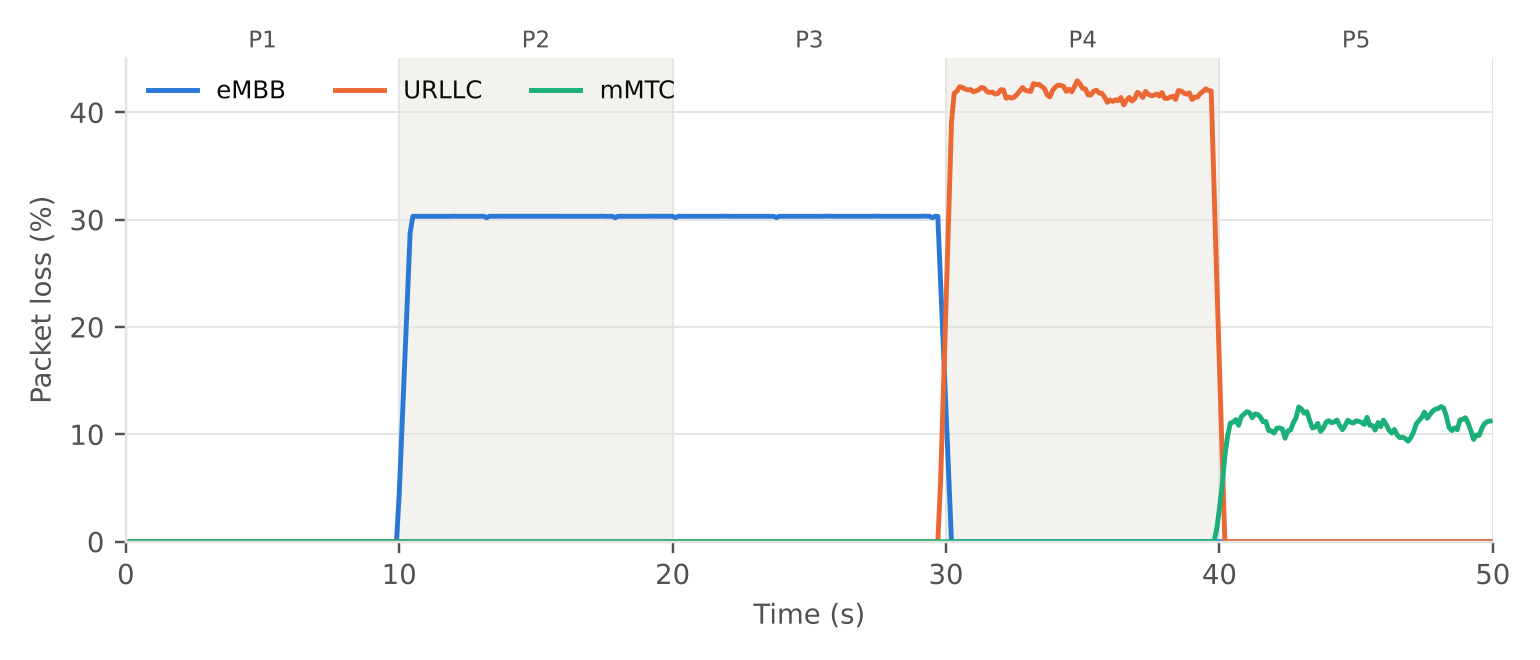
\includegraphics[width=\columnwidth]{fig4_packet_loss.png}
\caption{Packet loss per slice, computed by transmit interval.}
\label{fig:loss}
\end{figure}

\begin{figure}[t]
\centering
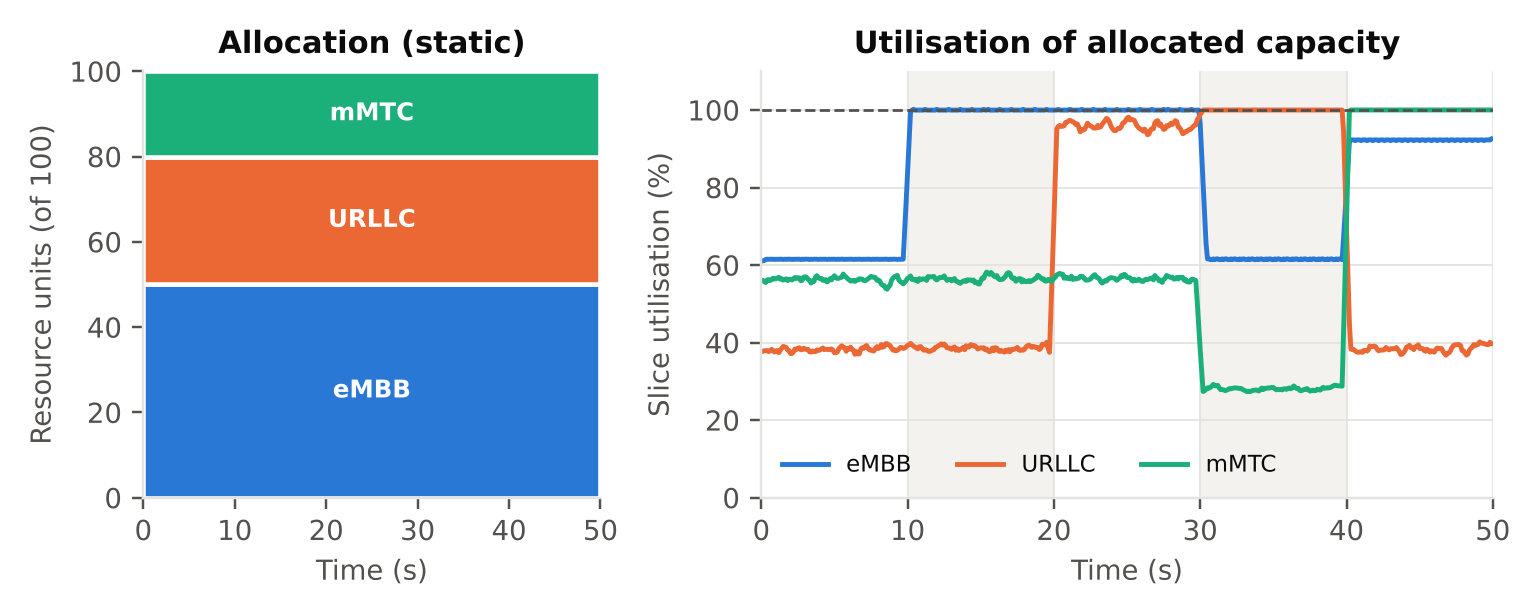
\includegraphics[width=\columnwidth]{fig5_allocation_utilisation.png}
\caption{Left: the static allocation. Right: utilisation of each slice's own capacity. Slices sit at 100\% while others are at 28 to 62\%.}
\label{fig:util}
\end{figure}

\begin{figure}[t]
\centering
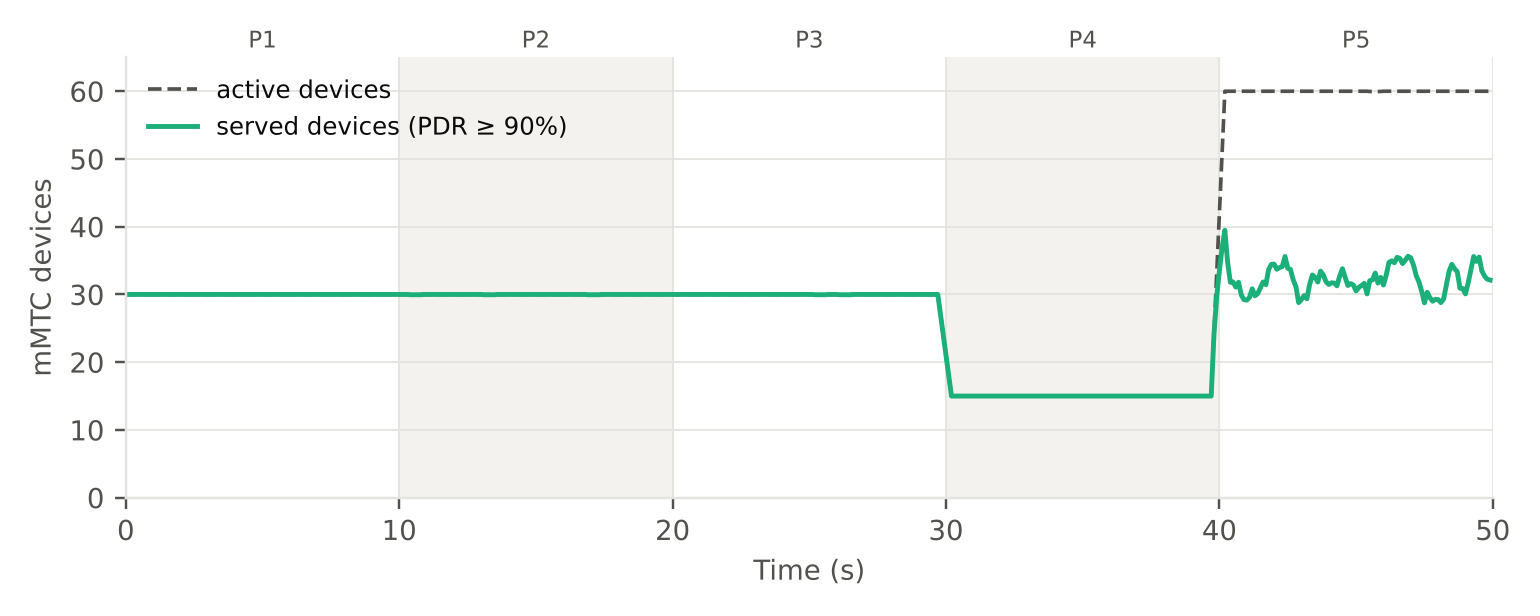
\includegraphics[width=\columnwidth]{fig6_mmtc_devices.png}
\caption{Active and served mMTC devices. In the surge only about half of the devices meet the 90\% delivery criterion.}
\label{fig:mmtc}
\end{figure}

\begin{figure}[t]
\centering
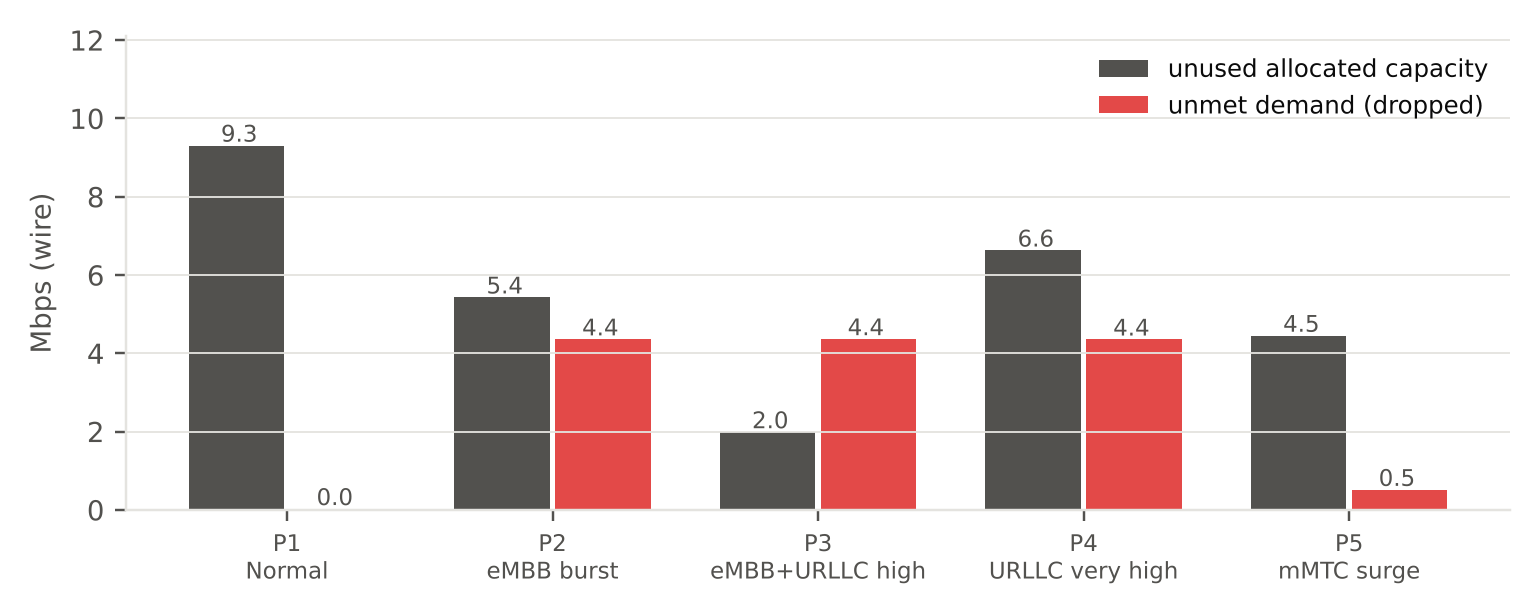
\includegraphics[width=\columnwidth]{fig7_stranded_capacity.png}
\caption{Per phase: capacity left unused in some slices versus demand dropped in others (wire Mbps, mean of 5 seeds).}
\label{fig:stranded}
\end{figure}

\begin{table*}[t]
\centering
\caption{Per-phase results of the static 50/30/20 allocation (mean over 5 seeds; $\pm$ is the 95\% CI where it is not negligible)}
\label{tab:summary}
\setlength{\tabcolsep}{4pt}
\resizebox{\textwidth}{!}{%
\begin{tabular}{@{}lcccccccccc@{}}
\toprule
& \multicolumn{2}{c}{eMBB} & \multicolumn{4}{c}{URLLC} & \multicolumn{2}{c}{mMTC} & \multicolumn{2}{c}{Pool} \\
\cmidrule(lr){2-3}\cmidrule(lr){4-7}\cmidrule(lr){8-9}\cmidrule(l){10-11}
Phase & loss (\%) & delay (ms) & delay (ms) & p95 (ms) & viol. (\%) & loss (\%) & served/active & loss (\%) & util. (\%) & idle / unmet (Mbps) \\
\midrule
P1 Normal & 0.0 & 2.5 & 1.52 & 1.9 & 0.0 & 0.0 & 30 / 30 & 0.0 & 53.5 & 9.3 / 0.0 \\
P2 eMBB burst & 29.6 & 99.0 & 1.52 & 1.9 & 0.0 & 0.0 & 30 / 30 & 0.0 & 72.9 & 5.4 / 4.4 \\
P3 eMBB + URLLC high & 30.3 & 100.5 & 4.9$\pm$0.5 & 7.4$\pm$0.6 & 9.5$\pm$2.8 & 0.0 & 30 / 30 & 0.0 & 90.1 & 2.0 / 4.4 \\
P4 URLLC very high & 0.0 & 5.9 & 32.1 & 32.4 & 99.9 & 41.8 & 15 / 15 & 0.0 & 66.9 & 6.6 / 4.4 \\
P5 mMTC surge & 0.0 & 3.2 & 1.85 & 2.2 & 1.2 & 0.0 & 32.5$\pm$0.5 / 60 & 11.0 & 77.7 & 4.5 / 0.5 \\
\bottomrule
\end{tabular}}
\end{table*}

\subsection{Model validation}
Before interpreting the results we check them against queueing theory. URLLC arrivals are the sum of three Poisson streams with fixed-size packets, so the URLLC pipe is an M/D/1 queue with service rate $\mu=6\,\text{Mbps}/(230\cdot 8\,\text{bits})=3261$ packets/s. The mean waiting time is $W_q=\rho/(2\mu(1-\rho))$. In P3, $\rho=5.75/6=0.958$ gives $W_q=3.5$~ms; adding 0.31~ms transmission and 1.12~ms of propagation and access delay predicts 4.95~ms, against a measured 4.92~ms. In P1 ($\rho=0.38$) the prediction is 1.52~ms, matching the measured 1.52~ms. When a pipe is overloaded, its FIFO stays full, and the delay should approach $B\cdot S/C_k$ for buffer $B=100$ packets of wire size $S$: 98.4~ms for eMBB, 30.7~ms for URLLC and 18.8~ms for mMTC. The measured values are 99.0 to 100.5, 32.1 and 19.4~ms; the 1 to 2~ms gap is propagation and transmission time. The simulation therefore behaves as a correctly implemented hard-partitioned queueing system.

\subsection{Observations per phase}
\textbf{P1 (normal):} all QoS targets are met, but 9.3~Mbps (46.5\%) of the pool is idle. The static partition is over-provisioned in quiet periods.

\textbf{P2 (eMBB burst):} eMBB offers 14.35~Mbps into a 10~Mbps pipe. Its queue fills, delay rises from 2.5 to 99~ms, and 29.6\% of eMBB packets are lost. At the same time URLLC and mMTC leave 5.4~Mbps idle, more than the 4.4~Mbps eMBB drops. A reallocation could have carried all eMBB traffic without harming the other slices.

\textbf{P3 (eMBB and URLLC high):} total offered load (22.4~Mbps) exceeds the pool, so some loss is unavoidable under any allocation. URLLC runs at 95.9\% of its pipe. Nothing is lost, but delay is high and variable: 9.5\% of URLLC packets miss the 10~ms budget. This shows that a slice can violate its latency target \emph{below} capacity, so a controller has to keep URLLC utilisation well below 100\%.

\textbf{P4 (URLLC very high):} URLLC offers 10.35~Mbps into a 6~Mbps pipe. 41.8\% of URLLC packets are lost and 99.9\% of delivered ones exceed the budget (32~ms delay). Meanwhile eMBB uses 62\% and mMTC 28\% of their pipes, leaving 6.6~Mbps idle against 4.4~Mbps of URLLC demand dropped. This is the clearest failure of static allocation, and the most damaging one because URLLC is the most critical slice.

\textbf{P5 (mMTC surge):} 60 devices offer 4.51~Mbps into a 4~Mbps pipe. Loss is 11.0\%, delay rises to 19.4~ms, and only 32.5 of 60 devices are served, while 4.5~Mbps is idle elsewhere. The 1.2\% URLLC violations in P5 are packets queued during P4 that are delivered just after the phase change.

\textbf{Overall:} averaged over the run, 27.8\% of the pool is idle and total utilisation is 72.2\%. In three of the five phases (P2, P4, P5) the dropped demand is smaller than the idle capacity, so the same total resources, divided differently, could have avoided the loss. These are the cases an adaptive controller is expected to improve. P3 is an overload case in which the controller can only choose \emph{which} slice absorbs the loss; a good policy should protect URLLC.

% =====================================================================
\section{Assumptions and Limitations}
\begin{itemize}
\item The radio access network is abstracted as rate pipes; there is no channel model, PHY/MAC scheduler or mobility. Resource units are not PRBs.
\item Slices are hard-isolated. Real deployments may let slices borrow idle resources; this baseline intentionally does not.
\item The 10~ms URLLC budget is a simulation choice that accounts for the modelled link delays; it is not the 3GPP radio-latency target.
\item Traffic is synthetic (CBR and Poisson) and uplink only. Results are specific to this scenario and buffer size; the 100-packet buffer directly sets the overload delays.
\item ns-3.44 was used for these runs; the code also targets ns-3.45.
\end{itemize}

% =====================================================================
\section{Conclusion and Future Work}
We built and validated an ns-3 network-slicing simulation with an enforced, run-time reconfigurable resource partition. With a static 50/30/20 split, the network simultaneously drops traffic and leaves capacity idle: up to 41.8\% URLLC loss with 99.9\% latency violations during a URLLC surge, about 30\% eMBB loss during eMBB bursts, half the mMTC devices unserved during a device surge, and 27.8\% of capacity unused on average. In three of five phases a different split of the same resources would have avoided the loss. Phase~2 will connect a DQN agent to \texttt{ApplyAllocation()} through ns3-ai, train it on randomised scenarios, and compare it with the static, random and heuristic baselines in the five planned experiments, followed by the Streamlit dashboard and the optional demand-forecasting extension.

% =====================================================================
\begin{thebibliography}{99}
\bibitem{itu2083} ITU-R, ``IMT Vision: Framework and overall objectives of the future development of IMT for 2020 and beyond,'' Recommendation ITU-R M.2083-0, Sep. 2015.
\bibitem{ts23501} 3GPP, ``System architecture for the 5G System (5GS),'' TS 23.501.
\bibitem{ts22261} 3GPP, ``Service requirements for the 5G system,'' TS 22.261.
\bibitem{foukas2017} X. Foukas, G. Patounas, A. Elmokashfi, and M. K. Marina, ``Network slicing in 5G: Survey and challenges,'' \emph{IEEE Commun. Mag.}, vol. 55, no. 5, pp. 94--101, 2017.
\bibitem{popovski2018} P. Popovski, K. F. Trillingsgaard, O. Simeone, and G. Durisi, ``5G wireless network slicing for eMBB, URLLC, and mMTC: A communication-theoretic view,'' \emph{IEEE Access}, vol. 6, pp. 55765--55779, 2018.
\bibitem{li2018} R. Li, Z. Zhao, Q. Sun, C.-L. I, C. Yang, X. Chen, M. Zhao, and H. Zhang, ``Deep reinforcement learning for resource management in network slicing,'' \emph{IEEE Access}, vol. 6, pp. 74429--74441, 2018.
\bibitem{mnih2015} V. Mnih \emph{et al.}, ``Human-level control through deep reinforcement learning,'' \emph{Nature}, vol. 518, pp. 529--533, 2015.
\bibitem{ns3} G. F. Riley and T. R. Henderson, ``The ns-3 network simulator,'' in \emph{Modeling and Tools for Network Simulation}, Springer, 2010, pp. 15--34.
\bibitem{lena2019} N. Patriciello, S. Lag\'en, B. Bojovi\'c, and L. Giupponi, ``An E2E simulator for 5G NR networks,'' \emph{Simulation Modelling Practice and Theory}, vol. 96, 2019.
\bibitem{ns3gym} P. Gaw{\l}owicz and A. Zubow, ``ns-3 meets OpenAI Gym: The playground for machine learning in networking research,'' in \emph{Proc. ACM MSWiM}, 2019.
\bibitem{ns3ai} H. Yin \emph{et al.}, ``ns3-ai: Fostering artificial intelligence algorithms for networking research,'' in \emph{Proc. Workshop on ns-3 (WNS3)}, 2020.
\bibitem{jain1984} R. Jain, D.-M. Chiu, and W. R. Hawe, ``A quantitative measure of fairness and discrimination for resource allocation in shared computer systems,'' DEC Research Report TR-301, 1984.
\end{thebibliography}

\end{document}
